\chapter{Metodologi dan Desain Sistem}

\section{Pengembangan Ontology}
Dari sepuluh tahap \textit{Methontology}, terdapat tiga tahap utama yang menghasilkan keluaran formal 
yaitu \textit{specification}, \textit{conceptualization} dan \textit{implementation}.
\par

\subsection{Specification}
Dalam tahap \textit{specification} pengembangan \textit{ontology}, terdapat tiga hal utama yang yang harus dideskripsikan yaitu domain, tujuan dan lingkup \textit{ontology}
yang dikembangkan.
\par
Tahap ini akan menghasilkan dokumen spesifikasi kebutuhan \textit{ontology} pada domain pariwisata. Tabel 3.1 adalah spesifikasi dari \textit{ontology} yang akan dibangun.

\begin{table}[h]
\begin{center}
\begin{tabular}{ |c|m{12cm}| } 
\hline
	Domain & Pariwisata \\
	\hline
	Tujuan & Ontology untuk merepresentasikan pengetahuan klasifikasi tujuan wisata dan aktivitas yang dapat dilakukan\\
	\hline
	Lingkup & Daftar kategori tujuan wisata, daftar tingkat kedekatan suatu tujuan wisata dengan kategori tujuan wisata, daftar kategori cuaca, daftar tujuan wisata,
	daftar atribut tujuan wisata. \\ 
	\hline
	Sumber & Wawancara dengan pakar. \newline 
	buku \textit{Tourism Planning, An Integrated and Sustainable Development Approach} karya Edward Inskeep. \\
	\hline
\end{tabular}
\end{center}
\caption{Tabel spesifikasi kebutuhan ontology yang akan dibangun}
\label{table2}
\end{table}

Domain dari \textit{ontology} yang dibuat berada di pariwisata, meliputi tujuan wisata dan kategorinya. Untuk bisa mengetahui bagaimana tujuan wisata dikategorikan,
maka perlu adanya konsultasi dengan pakar terkait dan studi pustaka pada buku rujukan yang direkomendasikan oleh pakar.

\subsection{Conceptualization}
Ketika tahap \textit{specification} telah selesai, maka akan didapat pengetahuan mengenai domain yang masih belum terstruktur dengan baik. Pada tahap {Conceptualization}, pengetahuan
yang tidak terstruktur tersebut akan diatur dengan representasi yang tidak bergantung pada bahasa pemrograman dan lingkungan \textit{runtime}\cite{lopez1999building}. 
\subsection{Implementation}

\section{Desain Sistem}
Sebelum masuk pada fase pengembangan sistem, menentukan desain kasar sistem merupakan hal yang krusial. Hal tersebut disebabkan karena memahami komponen apa saja yang ada pada sistem dan relasi antar komponen dapat membantu menentukan arah pengembangan sistem. 
 
\subsection{Arsitektur Sistem}
\par
Gambar 3.1 menjelaskan desain arsitektur sistem dan relasi-relasi antar komponen.
\newline
\begin{figure}[h!]
    \centering
    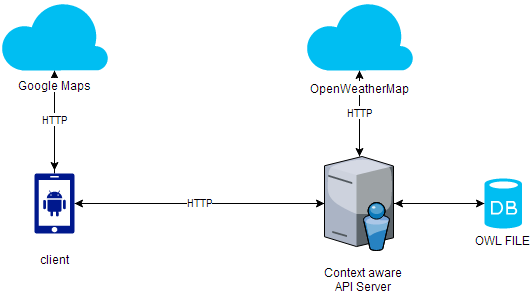
\includegraphics[scale=0.3]{img/arsitektur_sistem.png}
    \caption{Gambaran komponen-komponen sistem dan relasinya}
    \label{fig:Gambar}
\end{figure}

\par
Komponen-komponen RS yang akan dikembangkan penyusun terdiri dari \textit{client}, \textit{server}, basis data dengan fail OWL, Google Maps API dam OpenWeatherMap API. 
\textit{Client} berkomunikasi dengan Google Maps API untuk menampilkan data lokasi pengguna dan tujuan wisata. Selanjutnya \textit{client} mengirimkan \textit{HTTP request} ke 
\textit{server} dengan menyertakan data lokasi dan preferensi pengguna. Ketika \textit{server} menerima \textit{HTTP request}, \textit{server} akan membalas dengan 
\textit{HTTP response} yang berisi daftar rekomendasi tujuan wisata.

\subsection{Model Ontology}

Gambar 3.2 adalah garis besar model \textit{ontology} yang merepresentasikan pengetahuan sistem yang akan dibangun:
\begin{figure}[h!]
    \centering
    \includegraphics[scale=0.6]{img/ontology.png}
    \caption{Gambar \textit{ontology} representasi pengetahuan RS}
    \label{fig:Gambar}
\end{figure}
\newline
Struktur \textit{ontology} dibangun berdasarkan asumsi bahwa tempat wisata yang dapat dikunjungi ketika hujan juga dapat dikunjungi ketika cuaca cerah, tetapi tidak berlaku sebaliknya. Strukturnya juga menyimpan informasi mengenai lokasi dan waktu buka tempat wisata.
 
\subsection{Flowchart Sistem}
Secara umum, aliran kerja sistem dijelaskan pada gambar 3.3 dibawah ini:
\begin{figure}[h!]
    \centering
    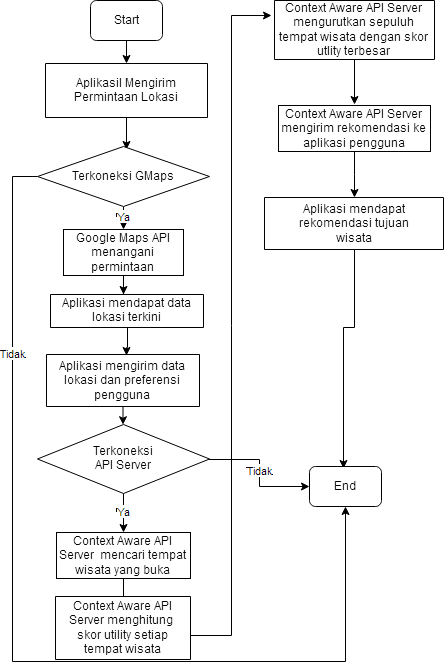
\includegraphics[scale=0.6]{img/flowchart-general.png}
    \caption{Gambaran aliran kerja sistem yang dikembangkan}
    \label{fig:Gambar}
\end{figure}
\textit{Flowchart} sistem pada gambar 3.3 dapat dijelaskan secara umum sebagai tiga kegiatan utama. Tiga kegiatan tersebut adalah mendapatkan alur mendapatkan informasi kontekstual dan preferensi tujuan wisata pengguna, melakukan \textit{reasoning} di \textit{web server} berdasar data yang masuk, dan mendapatkan rekomendasi tujuan wisata secara visual.
\section{Metodologi Pengembangan Sistem}

Tugas akhir ini akan disusun dengan melalui tahap-tahap berikut:
\begin{enumerate}

\item Desain Sistem
\par
Dalam tahap ini ada dua bagian, yaitu desain struktur \textit{ontology} dan pengembangan sistem.
\par
Tahap-tahap dalam mendesain struktur \textit{ontology} mengikuti \textit{Methontology} \cite{jones1998methodologies}, yaitu:
\begin{enumerate}
	\item Spesifikasi
	\item Akuisisi pengetahuan
	\item Konseptualisasi
	\item Integrasi
	\item Implementasi
	\item Evaluasi
	\item Dokumentasi
\end{enumerate} 
Berdasarkan lima komponen penting pada RS yang telah dijelaskan di gambar 3.1, berikut adalah langkah bagian pengembangan sistem yang akan ditempuh:
\begin{enumerate}
	\item Merancang GUI pada sisi \textit{client}.
	\item Merancang skema interaksi penggunaan aplikasi.
	\item Merancang format data yang dipertukarkan antara \textit{client} dan \textit{web server}.
	\item Merancang algoritma pada sisi \textit{client} dan \textit{web server}.
	\item Merancang \textit{query} untuk mengakuisisi pengetahuan pada data yang disimpan di \textit{SPARQL}.
\end{enumerate}

\item Pengumpulan Data Lokasi Wisata Bandung
\newline
Tujuan tahap ini adalah mendapatkan data lokasi wisata. Metode yang dapat dilakukan adalah:
\begin{enumerate}
	\item Observasi.
	Metode observasi dilakukan untuk mendapatkan data lokasi wisata yang tidak dikelola oleh pihak swasta.
	\item Wawancara pihak pengelola tempat wisata.
	Metode wawancara dilakukan untuk lokasi wisata yang dikelola oleh pihak swasta.
\end{enumerate}
\par
Tujuan dari tahap ini adalah mendapatkan data koordinat tujuan wisata di \textit{Google Maps}, analisis kondisi tujuan wisata pada cuaca cerah dan hujan, serta waktu ketika tujuan wisata dapat diakses.

\item Implementasi Sistem
\newline
Tahap implementasi meliputi:
\begin{enumerate}
	\item Pengembangan aplikasi Android.
	\item Pengembangan sisi \textit{server}.
	\item Implementasi komunikasi antar isi \textit{client} dan sisi \textit{server} serta \textit{client} dan \textit{Google Maps API}.
	\item Implementasi \textit{ontology} pada basis data \textit{SPARQL}.
\end{enumerate}
 
\item Pengujian
\newline
Tahap pengujian memiliki dua jenis pengujian:
\begin{enumerate}
	\item Pengujian utnuk menemukan \textit{bug}. Untuk menemukan \textit{bug}, sistem akan diuji coba dengan menggunakan skema \textit{white box}.
	\item Pengujian akurasi sistem. 
\end{enumerate}

\item Pembuatan Laporan
\newline 
Laporan akhir akan ditulis sesuai dengan kaidah dan ketetapan yang berlaku di institusi.
\end{enumerate}

